\documentclass{acm_proc_article-sp}

\begin{document}



\title{Beyond CRF Tagging for Web Search Query Understanding}
%\author{Ruiqiang Zhang Yi Chang\\
%Yahoo! Inc \\
%701 First Avenue, Sunnyvale, CA94089 }
%\date{}

%\numberofauthors{2}
%\author{
%\alignauthor
%Ruiqiang Zhang\\
% \affaddr{Yahoo! Inc}\\
% \affaddr{701 First Ave. }\\
% \affaddr{Sunnyvale, CA}\\
% \email{ruiqiang@yahoo-inc.com}
% 2nd. author
%\alignauthor
%\\Chikashi Nobata
% \affaddr{Yahoo! Inc}\\
% \affaddr{701 First Ave. }\\
% \affaddr{Sunnyvale, CA}\\
% \email{yichang@yahoo-inc.com}
%}

\maketitle

\begin{abstract}
Conditional Random Field (CRF) is a well-known machine learning approach and tagging of named entities with CRF achieves high tagging accuracy
However, in our Web search query intent understanding task, we found the CRF tagging also produced very high false positive results. In other words, CRF tagging generates too many bad interpretations that have to be rejected. This paper proposes a GBDT-based (Gradient Boosted Decision Tree) re-scoring method to re-rank the results generated by CRF tagger. The GBDT method is used as a classifier to recognize good or bad interpretations. We found this approach significantly reduced false positives and improved search user experience in online test. 
\end{abstract}



\section{Introduction}
Knowing query intent is an important factor for improving Web search user experience. If search engine can understand what users want to search for, search relevance can be improved.  In this work, one direct application of query intent understanding is to present user Web search results with Direct Display (DD) .  Rather than searching results from Web data, Direct Display search results from vertical content data such as Image, Local, Shopping or Movie if corresponding query intent is detected correctly. For example, if a query has Shopping intent, DD shows search results from Shopping listings.  Therefore, one pre-condition for DD is to understand query intent at a higher precision.



To understand query intent, our first step is to interpret query with predefined taxonomies. This step is called \emph{query interpretation} in this paper. Actually, this is a named entity recognition task. For this kind of task,  CRF method has the state-of-the-art performance in terms of accuracy over other methods like SVM, HMM and ME in sequence labeling.
However, we found this method had a higher false positive rate. To illustrate, we show some examples in Table~\ref{table:example}, where two queries and corresponding interpretations are shown. The interpretations are sorted according to the CRF tagging score $p(y|x)$ (will explain in the following sections). While the results contain excellent interpretations but also fair and bad ones. The problem we are facing is to detect the bad interpretations and reject them. Otherwise, DD will display worse results. 

We use GBDT\cite{Friedman:2002, Ye:2009} as the binary classifier to separate good interpretations from bad ones. GBDT is a regression model and  used after CRF tagging as a re-ranking method.
In the following sections, we will describe GBDT training, feature, and experiments. 










\begin{table*}
\begin{center}
\begin{tabular}{|c|c|c|c|c|} \hline
query & \# & interpretation & $p(y|x)$ & EGFB grade \\ \hline
napa & 1 &napa|ORGANIZATION(automobile) & 0.6 & E(xcellent)\\
& 2 &napa|PLACE(city) & 0.3 & E(xcellent) \\
& 3 &napa|TOKEN & $0.05$ & F(air) \\ \hline
dvd repair & 1 & (dvd repair)|PRODUCT & 0.45 & B(ad) \\
& 2 & dvd|PRODUCT repair|TOKEN & 0.4 & G(ood) \\
& 3 & dvd|TOKEN repair|TOKEN & 0.05 & F(air) \\
\hline
\end{tabular}
\caption{From CRF tagging: query interpretation, tagging scores and editorial evaluation grades}
\label{table:example}
\end{center}
\end{table*}

\section{Related Work}
According to some statistics, 85\% of query log queries contains one or more entities~\cite{Lin:2012}, which proves query NER is important for search. The work of \cite{Lin:2012} made research on finding actions by using entities inside queries.

Roughly speaking, techniques used in query understanding task include query segmentation and named entity recognition. 
\cite{Hagen:2012} described an overview of state-of-the-art works about query segmentation. Query segmentation is part of query interpretation task. According to \cite{Hagen:2012}, the best word segmentation results are around 85\%. 

The paper \cite{Guo:2009:NER} proposes a probabilistic approach to the named entity recognition using query log data and Latent Dirichlet Allocation. Topic model is constructed by a weakly supervised LDA method. The method is tested on a tag set with only 4 taxonomies related to medias. The best NER accuracy as reported is 80\%. However, the evaluation was based on known query segmentation. The number could be lower if query segmentation is unknown.



\section{Overview of CRF tagging model}


CRF approach has been studied for decades. The training and decoding methods used in this work have no much difference from the traditional methods, as pioneered by~\cite{lafferty:2001}. Therefore, we won't describe details about its theory. In short, 
CRF tagging model can be simply expressed as following formula,

\begin{equation}
p(y|x)=\frac{1}{Z(x)}\prod_{t=1}^{T}exp{\sum_{k=1}^{K}\theta_{k}f_{k}(y_{t},y_{t-1},x_{t})}
\label{eq:crf}
\end{equation}
For query interpretation task, $x$ and $y$ represent query sequence and taxonomy sequence respectively.

In the training stage, the model's parameter $\theta_{k}$ can be easily estimated by maximizing log likelihood of training data,

$$
\sum_{i=1}^{N}\sum_{t=1}^{T}\sum_{k=1}^{K}\theta_{k}f_{k}(y_{t}^{(i)},y_{t-1}^{(i)},x_{t}^{(i)})-\sum_{i=1}^{N}logZ(x^{(i)})
$$ 

CRF tagging includes entity boundary detection and taxonomy labeling. The two is completed in one step in this work. 
In the human labeled training data, entity boundary is tagged with ``B",``I" tags, indicating beginning/independent and intermediate position of an entity. Those tags are combined with a class name to indicate entity's span and category. For example, "B-organization I-organization" indicates a two term ORGANIZATION query. 

This work used many new features that is unique for query NER. Our model used about 30M features due to diversified web vocabulary and rich query context. We used the following information as features: precede/current/next query word, word position, word boundary, word spelling, lexical and query word topics. Topics were created by LDA (Latent Dirichlet Allocation) over 10 million queries. Our training data were selected randomly from query log and manually created by editors. 
In decoding stage, multiple interpretations can be produced and the order of interpretations can be ranked according to the value of $p(y|x)$. Usually, the top N-best results are used. 



We found using $p(y|x)$ as a criteria to select good interpretations was disappointed. An example is shown in Table~\ref{table:example}.
The table lists two example queries, ``napa" and ``dvd repair". The query ``napa" has two meanings, either organization name of automotive business or a city name of state California. While both of the top 2 interpretations in the table are correct, their $p(y|x)$ scores are very different. That makes hard to distinguish according to the value $p(y|x)$.
If we set threshold= $0.3$ so that both interpretation are chosen, the threshold is not appropriate for the second query, ``dvd repair" in which the first interpretation is a bad interpretation with a value above the threshold. Our CRF tagger mis-recognizes ``dvd repair" as a product at the first result, and assigned a probability of $0.45$. 
This interpretation will trigger Shopping DD if the first interpretation can't be rejected. Certainly, ``dvd repair" has no Shopping intent.



The above two examples show that we can't use $p(y|x)$ value to judge the interpretations.
We need another method to solve this problem. The new method can be a machine-learned classifier that have high performance to distinguish good and bad interpretations.
In this work, we used decision tree based classifier.


\section{GBDT rescoring model}



The re-scoring function is a logistic regression model. The probability is given by the formula below,

\begin{equation}
p(x) = \frac{1}{1+e^{(a*(b-f(x))}} \Longrightarrow y=\left \{\begin{array}{cc} +1 & p(x)\geqslant thrshld \\ -1 & othervise \end{array}\right.
\label{eq:gbdt}
\end{equation}

where $x$ is the generated feature vector for a given query and interpretation. $a$ and $b$ are the slope and pivot parameters. $a=2.0$ and $b=2.6$ are determined by optimizing classifier's performance in terms of recall and precision. $\{+1,-1\}$ denotes good interpretation and bad interpretation. $thrshld$ is set to separate good and bad interpretation according to the score $p(x)$. 

We employ Gradient Boosted Decision Tree algorithm 
to learn the function $f(x)$. Gradient Boosted Decision Tree is an
additive regression algorithm consisting of an ensemble of trees,
fitted to current residuals, gradients of the loss function, in a
forward step-wise manner. It iteratively fits an additive model as
%\begin{align}
$$
f_t(x) = T_t(x; \Theta) + \lambda \sum_{t=1}^T \beta_t T_t(x; \Theta_t)
$$
%\end{align}
\noindent such that certain loss function $L(y_i, f_T (x + i))$ is
minimized, where $T_t(x;\Theta_t)$ is a tree at iteration $t$,
weighted by parameter $\beta_t$, with a finite number of parameters,
$\Theta_t$ and $\lambda$ is the learning rate. At iteration t, tree
$T_t(x; \beta)$ is induced to fit the negative gradient by least
squares.


\noindent The optimal weights of trees $\beta_t$ are determined by
%\begin{align*}
$$
\beta_t = \text{argmin} _{\beta} \sum_i^N L(y_i, f_{t-1}(x_i) + \beta T(x_i, \theta))
$$
%\end{align*}

GBDT model is supervised machine learning. It needs manually created training data.
The process of creating training data is as follows. We randomly sampled hundreds of thousands of queries from Web search query log. For each query, we run CRF tagger to get top candidate interpretations. In addition, we generated more interpretations by maximum matching the entities defined in the lexicon. Editors assign 4 grades EGFB (Execllent, Good, Fair, Bad), to each of (query, interpretation) pairs. We show some examples on the last column of Table \ref{table:example}. 
Grade `E' is assigned to an excellent interpretation where all entities are correctly spanned and tagged. This interpretation will almost definitely lead to search results that are much better than those generated by the `default interpretation' (where all words are just `TOKEN').
Grade 1G' is assigned to a good interpretation where some entities but not all are correctly spanned and tagged. For example, some entities will not be tagged at all or tagged with a too general tag. This interpretation may lead to search results that are better than the default interpretation, but these could be further improved.
%This is a broad category that can range from only one tag being correct and all other tags tokens, to all tags being correct but one of them failing to go to the second %hierarchy level.
Grade `F' is the baseline grade and default level of interpretation. It is no better or worse than if each word was treated as an individual keyword match. Queries with all spans marked as ``token" are considered Fair. The exception to this rule is a query whose only interpretation are all spans labeled ``token". In this case, the interpretation is marked Good.
Grade `B' is a bad interpretation; some of the important entities are not spanned or tagged correctly, in a way that leads to a wrong understanding of the query.




\section{Features of GBDT}

GBDT is a tree model, its feature size is much smaller than CRF model. CRF model uses 30M features but our GBDT model has only 500 features. GBDT features can't be string value like CRF. Contextual features can't be used in GBDT. The 500 features are extracted from different sources. 

Eight features are from query level. (1) number of terms (2) number of stop words (3) number of special characters (4) number of entities recognized for this interpretation (5) number of non-tagged terms (6) number of non-token tags (7) position of first non-token tag (8) position of last non-token tag.

We defined 4 features from CRF tagger: (1) CRF raw probability (2) rank of CRF generated interpretation (3) ratio of current CRF interpretation to the top 1 CRF interpretation. (4) a boolean feature to indicate if interpretation is from CRF tagger.

There are two types of LM scores, context-independent tag (priors) and context dependent tag ngram LM scores. Context-independent tag scores are the average prior scores of any tags in the interpretation. Context-dependent tag sequence scores are ngram LM probability. Context-independent scores do not count token but context-dependent scores include tokens.
LM was built using editorial judgment data. 200 features are extracted by this method.

Some other features include template match. We manually wrote a lot of template-based rules to recognize query intents. These rules are from multiple domains. Take the query above as examples. (napa, PLACE) matches a Local template rule and (napa, ORGANIZATION) matches a Auto template rule. Features from template match include number of rule match.

Other features include counts of each taxonomy and ratio of each taxonomy if the query interpretation has multiple taxonomies. The feature size of this type is equal to the tag set. 

\section{Experiments}

We predefined an in-house taxonomy set. This set has two levels of granularity: coarse level and fine level. Coarse level has 20 categories and Fine level has 200 categories. The taxonomy was defined according to the business needs. For example, in order to differentiate Local query intent from Shopping query intent, our work defines two different categories: ORGANIZATION and BRAND while the two categories are not distinguished in others' work. For instance, ``apple" is an ORGANIZATION for the query ``apple store", and BRAND for ``apple iphone". ``apple store" has Local intent while ``apple iphone" has Shopping intent. The same ``apple" can have different intents by having both ORGANIZATION and BRAND in the taxonomy set. 

As documented in the previous sections, our whole query understanding system has two main models, CRF tagger and GBDT. The two models use different training data. CRF tagging model uses query perfect interpretation. GBDT model training uses 4-grade judgment. A few editors took two months to create 70k perfect interpretations and 200k EGFB data. 

The evaluation set is 7K randomly sampled queries from a search query log. They are manually labeled perfect interpretation. We use two metrics, Perfect@1 and Error@1, to evaluate system performance. Perfect@1 is the accuracy of perfect interpretation on the top 1 interpretations, calculated as ``the number of queries that have extract match with answers divided by the number of total queries". Each query has only one perfect interpretation. Error@1 is the error rate on top 1 interpretation, calculated as ``number of queries that has labeled incorrect entities on the top 1 interpretations divided by the number of total queries ". Note that Error@1 does not count unlabeled entities as errors. 

Table~\ref{table:pat1} shows the comparison between CRF tagger and GBDT. Both coarse level and fine level results are presented. CRF tagger has higher Perfect@1. It is a merit for using CRF tagger. But its Error@1 is also higher. That proves that CRF tagger can't directly be used for DD triggering. 
After GBDT rescoring, error rate is significantly reduced by 7\%. The results justified our efforts to introduce GBDT methods into query NER. But, from the table, we also observed Perfect@1 drop slightly after applied GBDT re-scoring. This can be explained as CRF tagger and GBDT function differently. CRF tagger can generate the most likely interpretations because it optimizes the likelihood of the training data. That is why it achieves higher p@1. Another reason is CRF tagger can integrate a great number of contextual features. GBDT is a regression model that maximizes EGFB grades.
It can make better judgment in classifying good and bad interpretations, but not good at generating good interpretations. After applying GBDT rescoring, while p@1 is slightly dropped, it is worthy because many bad interpretations are filtered. 






\begin{table}
\begin{center}
\begin{tabular}{|c|c|c|c|}
\hline
& CRF tagger & GBDT & change\\ \hline
Coarse Perfect@1 & 0.61 & 0.59 & -2\% \\
Coarse Error@1 & 0.25 & 0.19 & -6\%\\
Fine Perfect@1 & 0.50 & 0.49 & -1\%\\
Fine Error@1 & 0.29 & 0.22 & -7\%\\
\hline
\end{tabular}
\caption{Comparison of CRF tagger and GBDT in terms of Perfect@1 and Error@1}
\label{table:pat1}
\end{center}
\end{table}


The second test to compare CRF tagger and GBDT is to evaluate precision and recall of good interpretations. The test set is (query, interpretation) pairs evaluated with EGFB grades. The CRF tagger and GBDT model assign scores to each (query, interpretation) pair. A threshold can be set to determine the boundary of good and bad interpretation according to the score. Precision is calculated by the number of correctly detected E and G interpretations divided by the total number of recognized E/G interpretations. Recall is calculated by the number of correctly detected E and G interpretations divided by the total number of E and G interpretations of answers. The precision recall graph is shown in Fig.~\ref{fig:precision}. Each point is the precision and recall values corresponding to a threshold. The top green curve is of GBDT and the bottom blue curve is CRF tagger. We see GBDT is much better than CRF tagger in terms of both precision and recall. 


\begin{figure}
\centering
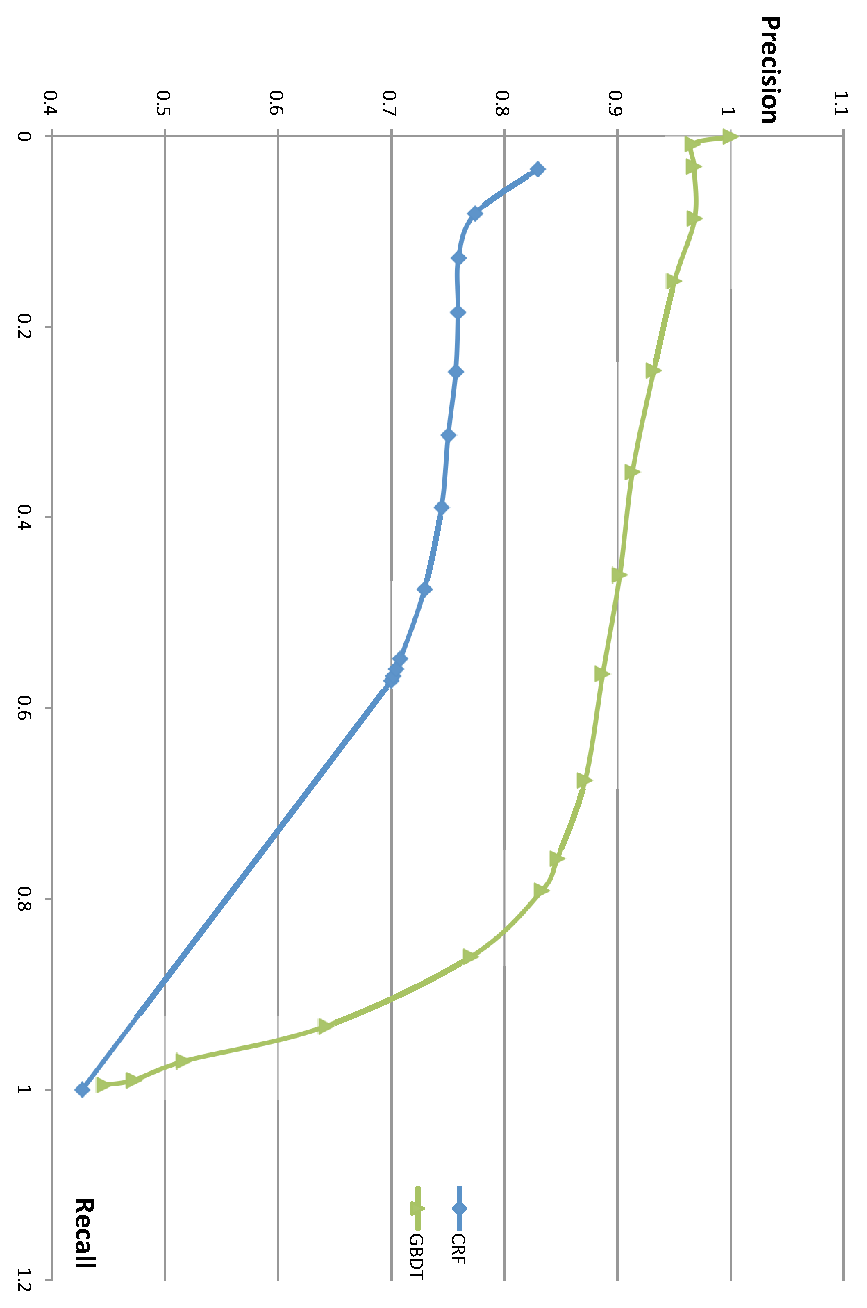
\epsfig{file=crf-gbdt-precision-recall.eps, height=3in, width=2in, angle=90}
\caption{Precision-recall comparison:CRF and GBDT}
\label{fig:precision}
\end{figure}



Query interpretation results are used to trigger DDs. The results were also evaluated by online user experience. Two buckets were used to compare CRF tagger and GBDT: the base bucket was run on CRF tagger and the test bucket on GBDT. We measured search result CTR(click through rate) for two weeks. CTR increases were observed significantly in all DDs such as Travel, Move, Local, Product, and Recipe. The highest CTR increase is 20\% for Movie DDs. 


We didn't find exactly matched references on query NER to compare with our work.Ttherefore we compared our system with two existing NER systems on different domain: Stanford NER~\footnote{http://nlp.stanford.edu/software/CRF-NER.shtml} and T-NER~\cite{Ritter:2011}. Table ~\ref{table:system comparison} lists results of all systems. Stanford NER was a supervised CRF tagger, trained using data from News domain. We applied it to our query domain evaluation data. Considering that queries in the data didn't have case information and also most of the queries were not proper sentences, it was not surprising that the results were much worse than ours. The second reference is T-NER, an NER for tweets. The query NER task is closer to tweet NER than news NER. The table lists the best results of T-NER from reference~\cite{Ritter:2011}. The comparison is based on three categories: PERSON, PLACE and ORGANIZATION. Our results are better than the two references. 

\begin{table}
\begin{center}
\begin{tabular}{|c|c|c|c|}
\hline
& Stanford NER & T-NER & Ours\\ \hline
PLACE & 0.18 & 0.74 & 0.86 \\ \hline
PERSON & 0.28 & 0.82 & 0.82 \\ \hline
ORGANIZATION & 0.01 & 0.66 & 0.67\\\hline
\end{tabular}
\caption{F1 performances for the three known NER systems }
\label{table:system comparison}
\end{center}
\end{table}

\section{Conclusions}
CRF tagging method is widely used in many named entity recognition tasks, for example, text, tweets and query. The paper is the first time to find the high false positive issue with this approach.
The issue may be not serious for other than query NER. But we found the issue impacted search engine query understanding seriously. 
This work proposed a solution to fix the weakness of CRF tagging by applying re-scoring GBDT models. 
It is found the integrated models by the two models derived the best results. This idea was validated though online user experiences test. 



\bibliographystyle{abbrv}

\bibliography{sigproc}



\end{document}




